\section{Einleitung} % (fold)
\label{sec:einleitung}

Eine Spannungsquelle ist hier ein Ger"at, welches "uber einen endlichen Zeitraum eine konstante elektrische Leistung liefern zu k"onnen. In diesem Versuch werden die Leerlaufspannung und der Innenwiderstand von Spannungsquellen gemessen, um das Verhalten innerhalb einer elektrischen Schaltung beschreiben zu k"onnen.

\section{Theorie} % (fold)
\label{sec:theorie}


\subsection{Leerlaufspannung} % (fold)
\label{sub:leerlaufspannung}

Die Leerlaufspannung $U_\mathrm{0}$ liegt an den Ausgangsklemmen einer Spannungsquelle an, wenn kein Strom entnommmen wird.

\subsection{Innenwiderstand} % (fold)
\label{sub:klemmenspannung}

Flie"st ein endlicher Strom $I$ durch Anschluss eines Lastwiderstandes $R_\mathrm{a}$, sinkt die Klemmenspannung $U_\mathrm{k}$ auf einen Wert unterhalb von $U_\mathrm{0}$.

Dies ist erkl"arbar, wenn der Spannungsquelle ein Innenwiderstand $R_\mathrm{i}$ zugeordnet wird.

\subsection{Ersatzschaltbild} % (fold)
\label{sub:ersatzschaltbild}

\begin{wrapfigure}{r}{7cm}
	\centering
	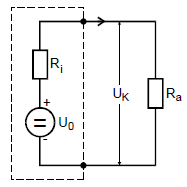
\includegraphics[width = 7cm]{img/Monozelle.PNG}
	\caption{Ersatzschaltbild einer realen Spannungsquelle mit Lastwiderstand $R_\mathrm{a}$ \cite{anleitung}.}
	\label{monozelle}
\end{wrapfigure}

Der gestrichelte Bereich in Abb. \ref{monozelle} wird als Ersatzschaltbild einer realen Spannngsquelle verwendet.
Es besteht aus einer idealen Spannungsquelle, welche eine Leerlaufspannung $U_\mathrm{0}$ liefert, und einem dazu in Reihe geschaltetem ohmschen Widerstand $R_\mathrm{i}$.

\subsection{Direkte Messung der Leerlaufspannung} % (fold)
\label{sub:direkte_messung_der_leerlaufspannung}

Das zweite Kirchhoffschen Gesetz lautet:

\begin{equation}
	\sum_n U_\mathrm{0,n} = \sum_m R_\mathrm{m} I_\mathrm{m} \qquad . \label{kirch}
\end{equation}

F"ur das vorliegende Problem in Abb. \ref{monozelle} ergibt sich aus \eqref{kirch}:

\begin{eqnarray}
	U_\mathrm{0} &=& I R_\mathrm{i} + I R_\mathrm{i} \qquad , \nonumber \\
	U_\mathrm{k} = I R_\mathrm{a} &=& U_\mathrm{0} - I R_\mathrm{i} \qquad . \label{uk}
\end{eqnarray}

Daraus folgt, dass mit zunehmendem Strom $I$ die Klemmenspannung $U_\mathrm{k}$ absinkt.
Zudem ergibt sich, dass zu einer direkten Messung der Leerlaufspannung $U_\mathrm{0}$ ein hochohmiges Voltmeter erforderlich ist. Im falle eines kleinen Stromes kann so der Term $I R_\mathrm{i}$ in Gleichung \eqref{uk} vernachl"assigt werden, sodass gilt $U_\mathrm{k} \approx U_\mathrm{0}$.

\subsection{Leistungsanpassung} % (fold)
\label{sub:leistungsanpassung}

Der Innenwiderstand $R_\mathrm{i}$ bewirkt, dass sich keine beliebig hohe Leistung der Spannungsquelle entnehmen l"asst.

F"ur die Leistung ergibt sich:

\begin{equation}
	N(R_\mathrm{a}) = I^2 R_\mathrm{a} = \frac{{U_\mathrm{0} }^2 R_\mathrm{a}}{{(R_\mathrm{a} + R_\mathrm{i})}^2} \qquad .
\end{equation}

Die Leistung $N(R_\mathrm{a})$ durchl"auft ein Maximum bei $R_\mathrm{a,max} = R_\mathrm{i}$.
Ist gerade $R_\mathrm{a} = R_\mathrm{a,max}$ gew"ahlt, so wird von Leistungsanpassung gesprochen.

In der Nachrichten- und Messtechnik wird davon viel Gebrauch gemacht.
In der Starkstromtechnik hingegen besitzt dies einige Nachteile, da der Innenwiderstand von z.B. RC-Generatoren oder elektronisch geregelten Spannungskonstanthaltern nicht unbedingt dich den Gleichstromwiderstand gegeben ist.
In einem solchen Fall ist es notwendig den Innenwiderstand als differentielle Gr"o"se einzuf"uhren:

\begin{equation}
	R_\mathrm{i} = \frac{\mathrm{d}U_\mathrm{k}}{\mathrm{d}I} \qquad .
\end{equation}